\chapter{F018-compatibele controller voor Direct Memory Access (DMA)}
\label{cha:dmagic}

De MEGA65 bevat een F018/F018A-compatibele DMA-controller. Anders dan in de C65, waar de DMA-controller als een afzonderlijke chip bestaat, maakt deze in de MEGA65 deel uit van de 45GS02-processor. Omdat het gebruik van de DMA-controller echter een logisch afzonderlijk onderwerp vormt, wordt het apart in deze bijlage besproken.

De DMA-controller van de MEGA65 biedt diverse belangrijke verbeteringen ten opzichte van de F018/F018A-DMAgic-chips van de C65:

\begin{itemize}
\item{\bf Snelheid} De MEGA65 voert DMA-bewerkingen uit met 40 MHz, waardoor per seconde 40 MB kan worden gevuld of 20 MB kan worden gekopieerd. Zo is het bijvoorbeeld mogelijk om een volledige bitmapafbeelding van 8 KB in C64-stijl in circa 200 microseconden te kopiëren, wat overeenkomt met minder dan vier rasterlijnen! \item{\bf Toegang tot het volledige geheugen} De DMA-controller van de MEGA65 biedt toegang tot alle 256 MB van de adresruimte. \item{\bf Ondersteuning voor het kopiëren van texturen} De DMA-controller van de MEGA65 kan fractionele adresberekeningen uitvoeren ter ondersteuning van hardwarematige textuurschaling, evenals adresstriding, waardoor het in principe mogelijk is om een textuur gelijktijdig te schalen en vanuit het geheugen naar het scherm te tekenen. Dat zou nuttig zijn als iemand gek genoeg zou zijn om een spel in de stijl van Wolfenstein of Doom op de MEGA65 te implementeren. \item{\bf Ondersteuning voor transparantie- en maskerwaarden} De DMA-controller van de MEGA65 kan de opdracht krijgen om bij het kopiëren van geheugen een speciale waarde te negeren, waardoor de inhoud van het bestemmingsgeheugen ongewijzigd blijft. Dit maakt het maskeren van transparante gebieden bij een DMA-kopie mogelijk, wat het blitten van grafische vormen aanzienlijk vereenvoudigt. \item{\bf Optielijst per taak} Voor elke taak in een geketende lijst van DMA-taken kunnen diverse opties worden geconfigureerd, zoals het selecteren van de F018- of F018B-modus, het wijzigen van de transparantiewaarde, fractionele adresstappen of het bron- of bestemmingsgeheugengebied.

\item{\bf Achtergrond-audio-DMA}  De MEGA65 beschikt over mogelijkheden voor achtergrond-audio-DMA, vergelijkbaar met de Amiga\texttrademark{}-serie computers. Belangrijke verschillen zijn dat de MEGA65 samples van 8 of 16 bits kan gebruiken, zeer hoge samplerates tot ongeveer 1 MHz ondersteunt, 256 volume-instellingen per kanaal heeft en geen modulatie tussen de kanalen kent.

\end{itemize}


\section{F018A/B-DMA-taken}

Om een DMA-taak met de F018-serie DMA-controllers uit te voeren, moet u de lijst met DMA-taken in het geheugen opbouwen en vervolgens het adres van deze lijst in de DMA-adresregisters schrijven. De DMA-taak wordt uitgevoerd wanneer u naar het register ADDRLSBTRIG (\$D700) schrijft. Om die reden moet u eerst het MSB en het banknummer van de DMA-lijst in \$D701 en \$D702 schrijven en pas daarna het LSB, nadat u deze beide registers hebt ingesteld. Indien u met dezelfde lijststructuur in het geheugen meerdere DMA-taken wilt uitvoeren, kunt u gewoon opnieuw naar ADDRLSBTRIG schrijven nadat u de inhoud van de lijst hebt bijgewerkt, mits geen ander programma de inhoud van \$D701 of \$D702 heeft gewijzigd. Houd er rekening mee dat BASIC 65 de DMA-controller gebruikt om het scherm te laten scrollen. Het is dan ook doorgaans het veiligst om altijd naar alle drie de registers te schrijven.

Nadat er naar ADDRLSBTRIG is geschreven, wordt de DMA-taak onmiddellijk afgerond. Anders dan in de C65 maakt de DMA-controller in de MEGA65 deel uit van de processor. Dit betekent dat de processor stopt met het uitvoeren van instructies totdat de DMA-taak is voltooid. De enige uitzondering hierop is dat audio-DMA doorgaat en cycli onttrekt aan elke andere DMA-activiteit, zodat de geluidsweergave niet wordt beïnvloed.

Dit gedrag betekent dat DMA-taken, anders dan op de C65, niet kunnen worden onderbroken. Heeft uw programma gevoelige timingvereisten, dan moet u grotere DMA-taken wellicht opsplitsen in verscheidene kleinere taken. Deze zorg wordt enigszins gecompenseerd door de hoge snelheid van de DMA in de MEGA65, die per seconde 40.5 MB geheugen kan vullen en 20.25 MB kan kopiëren, vergeleken met circa 3.5 MB en 1.7 MB per seconde op een C65. Daardoor kunnen grotere DMA-taken worden uitgevoerd zonder dat u zich zorgen hoeft te maken over de gevolgen voor realtime-elementen van een programma. Zo is het bijvoorbeeld mogelijk om met de DMA-controller van de MEGA65 een tekstscherm van 80 kolommen bij 50 rijen te vullen in slechts 200 microseconden.

\subsection{Indeling van de F018-DMA-taaklijst}

De DMA-controller van de MEGA65 ondersteunt de twee formaten voor DMA-taaklijsten die de oorspronkelijke F018 gebruikte, welke in de vroege C65-prototypen werd toegepast (tot revisie 2B), en die de F018B en latere revisies gebruikten, welke in de C65-prototypen van revisie 3 -- 5 werden toegepast. Het belangrijkste verschil is de toevoeging van een tweede commandobyte, zoals de volgende tabellen tonen:

Het is belangrijk om te weten welke stijl de DMA-controller verwacht. De Hypervisor van de MEGA65 stelt de modus in op basis van de gedetecteerde versie van de C65-ROM, indien er één wordt uitgevoerd. Indien het een oudere versie betreft, wordt de F018-stijl verwacht; anders wordt de nieuwere F018B-stijl verwacht. U kunt nagaan welke stijl is geselecteerd door bit 0 van \$D703 op te vragen: staat deze op 1, dan wordt het nieuwere F018B-lijstformaat van 12 bytes verwacht; staat deze op 0, dan wordt het oudere F018-lijstformaat van 11 bytes verwacht. De verwachte stijl kan worden ingesteld door naar dit register te schrijven.

Tenzij u software schrijft die ook op een C65-prototype moet draaien, kunt u waarschijnlijk het beste gebruikmaken van de Enhanced DMA-taken van de MEGA65, waarvan het lijstformaat expliciet in de lijst zelf wordt opgegeven. Omdat de Enhanced DMA-taken een uitbreiding zijn van de F018/F018B-DMA-taken, moet u het volgende toch lezen, tenzij u het gedrag van de F018-DMA-controller al kent.

\subsubsection{Structuur van de 11-byte F018-DMA-lijst}
\begin{center}
\begin{tabular}{|>{\centering\arraybackslash}p{1.5cm}|p{8cm}|}
  \hline
Offset & Inhoud \\
  \hline
\$00 & Commando LSB \\  \$01 & Aantal LSB \\  \$02 & Aantal MSB \\  \$03 & Bronadres LSB \\  \$04 & Bronadres MSB \\  \$05 & Bronadres BANK en FLAGS \\  \$06 & Bestemmingsadres LSB \\  \$07 & Bestemmingsadres MSB \\  \$08 & Bestemmingsadres BANK en FLAGS \\  \$09 & Modulo LSB \\  \$0a & Modulo MSB \\
  \hline
\multicolumn{2}{p{9.5cm}}{* Het commando-MSB is \$00 bij gebruik van dit lijstformaat.}

\end{tabular}
\end{center}

\subsubsection{Structuur van de 12-byte F018B-DMA-lijst}
\begin{center}
\begin{tabular}{|>{\centering\arraybackslash}p{1.5cm}|p{8cm}|}
  \hline
Offset & Inhoud \\
  \hline
\$00 & Commando LSB \\  \$01 & Aantal LSB \\  \$02 & Aantal MSB \\  \$03 & Bronadres LSB \\  \$04 & Bronadres MSB \\  \$05 & Bronadres BANK en FLAGS \\  \$06 & Bestemmingsadres LSB \\  \$07 & Bestemmingsadres MSB \\  \$08 & Bestemmingsadres BANK en FLAGS \\  \$09 & Commando MSB \\  \$0a & Modulo LSB / Modus \\  \$0b & Modulo MSB / Modus \\
  \hline
\end{tabular}
\end{center}

De structuur van het commandowoord is als volgt:
\begin{center}
\begin{tabular}{|>{\centering\arraybackslash}p{1.5cm}|p{8cm}|}
  \hline
Bit(s) & Inhoud \\
  \hline
0 -- 1 & DMA-bewerkingstype \\  2 & Ketting (d.w.z. er volgt nog een DMA-lijst) \\  3 & Toegeven aan interrupts \\  4 & MINTERM -SA,-DA bit \\  5 & MINTERM -SA,DA bit \\  6 & MINTERM SA,-DA bit \\  7 & MINTERM SA,DA bit \\  8 -- 9 & Adresseermethode van de bron \\  10 -- 11 & Adresseermethode van de bestemming \\  12 -- 15 & GERESERVEERD. Altijd op 0 instellen \\
  \hline
\end{tabular}
\end{center}

Het commando-veld kent de volgende vier waarden:
\begin{center}
\begin{tabular}{|>{\centering\arraybackslash}p{1.5cm}|p{8cm}|}
  \hline
  Waarde & Inhoud \\
  \hline
  \%00 (0) & Kopiëren \\  \%01 (1) & Mengen (via MINTERMs) \\  \%10 (2) & Wisselen \\  \%11 (3) & Vullen \\
  \hline
  \multicolumn{2}{p{9.5cm}}{* Alleen Kopiëren en Vullen zijn op het moment van schrijven geïmplementeerd.}
\end{tabular}
\end{center}

De velden voor de adresseermethode kennen de volgende vier waarden:

\begin{center}
  \begin{tabular}{|>{\centering\arraybackslash}p{1.5cm}|p{8cm}|}
  \hline
  Waarde & Inhoud \\
  \hline
  \%00 (0) & Lineair (normaal) adresseren \\  \%01 (1) & Modulo (rechthoekig) adresseren \\  \%10 (2) & Vasthouden (constant adres) \\  \%11 (3) & XY MOD (rechthoekige bitmap) adresseren \\
  \hline
  \multicolumn{2}{p{9.5cm}}{* Alleen Lineair, Modulo en Vasthouden zijn op het moment van schrijven geïmplementeerd.}
\end{tabular}
\end{center}

Het BANK- en FLAGS-veld voor de bron- en bestemmingsadressen maakt het mogelijk adressen binnen een adresruimte van 1 MB te selecteren. Om geheugen buiten de eerste 1 MB te benaderen, is het noodzakelijk een Enhanced DMA-taak te gebruiken met de juiste optiebytes om de MB van het bron- en/of bestemmingsgeheugen te selecteren. Het BANK- en FLAGS-veld heeft de volgende structuur:

\begin{center}
\begin{tabular}{|>{\centering\arraybackslash}p{1.5cm}|p{8cm}|}
  \hline
  Bit(s) & Inhoud \\
  \hline
  0 -- 3 & Geheugenbank binnen de geselecteerde MB \\  4 & HOLD, d.w.z. wijzig het adres niet \\  5 & MODULO, d.w.z. pas het MODULO-veld toe voor de wrap-around binnen een beperkte geheugenruimte \\  6 & DIRECTION. Indien gezet, wordt het adres verlaagd in plaats van verhoogd. \\  7 & I/O. Indien gezet, zijn de I/O-registers tijdens de DMA zichtbaar op \$D000 -- \$DFFF. \\
  \hline
\end{tabular}
\end{center}

\subsubsection{Eenvoudige DMA-bewerkingen uitvoeren}

Voor informatie over het gebruik van de DMA-controller vanuit BASIC 65, zie de BASIC-opdracht \stw{DMA} in \bookvref{BASIC 65 Commands!DMA}.

Om de DMA-controller vanuit assembleertaal te gebruiken, bouwt u een gegevensstructuur met de DMA-lijst en stelt u daarna \$D702 -- \$D700 in op het adres van de lijst. Om bijvoorbeeld het scherm in de C65-modus te wissen door het met spaties te vullen, zou de volgende routine kunnen worden gebruikt:

\begin{asmcodesmall}
  ; De DMA-lijst bevindt zich in BANK 0
  LDA #$00
  STA $D702
  ; Stel het MSB van het DMA-lijstadres in
  LDA #>dmalist
  STA $D701
  ; Stel het LSB van het DMA-lijstadres in en voer de DMA uit
  LDA #<dmalist
  STA $D700
  RTS

dmalist:
  .byte $03   ; Commando-laagbyte: FILL
  .word 2000  ; Aantal: 80x25 = 2000 bytes
  .word $0020 ; Vul met waarde $20
  .byte $00   ; Bronbank (genegeerd bij een FILL-bewerking)
  .word $0800 ; Bestemmingsadres van de schermgegevens
  .byte $00   ; Het scherm bevindt zich in bank 0
  .byte $00   ; Commando-hoogbyte
  .word $0000 ; Modulo (genegeerd vanwege het gekozen commando)
\end{asmcodesmall}

Het is ook mogelijk meer dan één DMA-taak tegelijk uit te voeren door de CHAIN-bit in het lage byte van het commando te zetten. Om bijvoorbeeld het scherm te wissen zoals hiervoor en daarnaast ook het kleurengeheugen (colour-RAM) van het scherm te wissen, zou u iets kunnen gebruiken als:

\begin{asmcodesmall}
  ; De DMA-lijst bevindt zich in BANK 0
  LDA #$00
  STA $D702
  ; Stel het MSB van het DMA-lijstadres in
  LDA #>dmalist
  STA $D701
  ; Stel het LSB van het DMA-lijstadres in en voer de DMA uit
  LDA #<dmalist
  STA $D700
  RTS

dmalist:
  .byte $07   ; Commando-laagbyte: FILL + CHAIN
  .word 2000  ; Aantal: 80x25 = 2000 bytes
  .word $0020 ; Vul met waarde $20
  .byte $00   ; Bronbank (genegeerd bij een FILL-bewerking)
  .word $0800 ; Bestemmingsadres van de schermgegevens
  .byte $00   ; Het scherm bevindt zich in bank 0
  .byte $00   ; Commando-hoogbyte
  .word $0000 ; Modulo (genegeerd vanwege het gekozen commando)

  ; De tweede DMA-taak volgt direct op de eerste
  .byte $03   ; Commando-laagbyte: FILL
  .word 2000  ; Aantal: 80x25 = 2000 bytes
  .word $0001 ; Vul met waarde $01 = wit
  .byte $00   ; Bronbank (genegeerd bij een FILL-bewerking)
  .word $F800 ; Bestemmingsadres van het kleurengeheugen
  .byte $01   ; Het kleurengeheugen bevindt zich in
              ; bank 1 ($1F800-$1FFFF)
  .byte $00   ; Commando-hoogbyte
  .word $0000 ; Modulo (genegeerd vanwege het gekozen commando)
\end{asmcodesmall}

Geheugen kopiëren lijkt sterk op het vullen van geheugen, met dit verschil dat het lage byte van het commando moet worden aangepast en dat het bronadresveld correct moet worden geïnitialiseerd. Om bijvoorbeeld de tekenset uit de ROM op \$2D000 -- \$2DFFF te kopiëren naar \$5000, zou u iets kunnen gebruiken als:

\begin{asmcodesmall}
  ; De DMA-lijst bevindt zich in BANK 0
  LDA #$00
  STA $D702
  ; Stel het MSB van het DMA-lijstadres in
  LDA #>dmalist
  STA $D701
  ; Stel het LSB van het DMA-lijstadres in en voer de DMA uit
  LDA #<dmalist
  STA $D700
  RTS

dmalist:
  .byte $00   ; Commando-laagbyte: COPY
  .word $1000 ; Aantal: 4KB = 4096
  .word $D000 ; Kopieer vanaf $xD000
  .byte $02   ; Bronbank = $02 voor $2xxxx
  .word $5000 ; Bestemmingsadres van de schermgegevens
  .byte $00   ; Het scherm bevindt zich in bank 0
  .byte $00   ; Commando-hoogbyte
  .word $0000 ; Modulo (genegeerd vanwege het gekozen commando)
\end{asmcodesmall}

Het is ook mogelijk vanuit BASIC 2 in de C64-modus een DMA-bewerking uit te voeren door de benodigde waarden met POKE te schrijven, nadat u er eerst voor hebt gezorgd dat de MEGA65- of C65-I/O-modus is geselecteerd door de juiste waarden naar \$D02F (53295) te schrijven. Om bijvoorbeeld het scherm in C64 BASIC 2 te wissen met behulp van de DMA-controller, zou u iets kunnen gebruiken als:

\begin{tcolorbox}[colback=black,coltext=white]
\verbatimfont{\codefont}
\begin{verbatim}
10 rem schakel de MEGA65-I/O in
20 poke53295,asc("g"):poke53295,asc("s")
30 rem DMA-lijst in data-regels
40 data 3: rem commando-lsb = vullen
50 data 232,3 : rem scherm is 1000 bytes = 3*256+232
60 data 32,0: rem vullen met spatie = 32
70 data 0: rem bronbank (niet gebruikt bij vullen)
80 data 0,4: rem schermadres = 1024 = 4*256
90 data 0: rem scherm bevindt zich in bank 0
100 data 0: rem hoge byte van commando
110 data 0,0: rem modulo (niet gebruikt in deze opgave)
120 rem zet de DMA-lijst op $c000 = 49152
130 fori=0to11:reada:poke49152+i,a:next
140 rem voer de taak uit
150 poke55042,0: rem DMA-lijst staat in bank 0
160 poke55041,192: rem DMA-lijst staat in $c0xx
170 poke55040,0: rem DMA-lijst staat in $xx00, en voer uit
\end{verbatim}
\end{tcolorbox}


Hoewel dit elke keer vrij omslachtig is, hoeft u, indien u het scherm opnieuw wilt wissen, niets anders te doen dan opnieuw \stw{POKE 55040,0} uit te voeren, ervan uitgaande dat de DMA-lijst en de registers van de DMA-controller niet zijn gewijzigd sinds de vorige keer dat de DMA-taak is uitgevoerd.

De HOLD-, I/O- en andere opties kunnen ook worden gebruikt om interessante effecten te bereiken. Om bijvoorbeeld zeer snel een nieuwe waarde naar de achtergrondkleur van het scherm te schrijven, kunt u een geheugengebied kopiëren naar \$D021, met de I/O-vlag gezet zodat het I/O-register in de DMA-taak zichtbaar wordt voor schrijven, en de HOLD-vlag gezet zodat herhaaldelijk naar hetzelfde adres wordt geschreven. Hiermee wordt met een snelheid van 20.5 MHz naar de achtergrondkleur geschreven, bijna zo snel als de videopixelklok (27 MHz). Zo kunnen wij de kleur vrijwel per pixel wijzigen.

Met een beetje zorg kunnen wij deze routine zo maken dat de uitvoering ervan precies één rasterlijn duurt en zo verticale rasterbalken trekken, of een soort frankenstein-videomodus creëren die een lineaire geheugenindeling gebruikt -- ten koste van alle verwerkingstijd gedurende het actieve deel van het beeld.

Het volgende voorbeeld doet dit om verticale rasterbalken op het scherm te trekken. Het programma gaat ervan uit dat de MEGA65 op PAL is ingesteld. Voor NTSC moet de omvang van de DMA-overdracht enigszins worden verkleind. Verder valt bij dit programma op dat met MEGA65 Enhanced-DMA-optie \$81 de bestemmingsmegabyte van het geheugen op \$FFxxxxx wordt ingesteld, de bank op \$D en het bestemmingsadres op \$0021, om zo het volledige adres \$FFD0021 te vormen. Dit is de werkelijke locatie van het randkleurregister van de VIC-IV. Het programma is geschreven met ACME-compatibele syntaxis.

\begin{asmcodesmall}
basicheader:
  ;; 2020 SYS 2061
  !word $80A,2020
  !byte $9E,$32,$30,$36,$31,0,0,0

  ;; Werkelijke code begint op $080d = 2061
main:
  SEI
  LDA #$47      ; Schakel de MEGA65-I/O in
  STA $D02F
  LDA #$53
  STA $D02F
  LDA #65       ; Stel de CPU-snelheid in op snel
  STA 0
  LDA #0        ; Schakel het scherm uit, alles is schermrandkleur
  STA $D011

  LDA $D012     ; Wacht tot het begin van de volgende rasterlijn
raster_sync:    ; vóór het begin van de lus voor horizontale
  CMP $D012     ; uitlijning
  BEQ raster_sync

  ;; De volgende lus duurt precies één rasterlijn
  ;; bij 40,5 MHz in PAL
loop:
  JSR triggerdma
  JMP loop

triggerdma:
  LDA #0      ; Zorg dat het F018-lijstformaat actief is
  STA $D703

  LDA #0      ; DMA-lijstbank
  STA $D702
  LDA #>rasterdmalist
  STA $D701
  LDA #<rasterdmalist
  STA $D705
  RTS
\end{asmcodesmall}

\begin{asmcodesmall}
rasterdmalist:
  !byte $81,$FF,$00
  !byte $00     ; COPY
  !word 619     ; De DMA-overdracht is 619 bytes lang
  !word rastercolours  ; bronadres
  !byte $00     ; bronbank
  !word $0020   ; bestemmingsadres
  !byte $1D     ; bestemmingsbank + HOLD
  ;; ongebruikt moduloveld
  !word $0000
\end{asmcodesmall}

\begin{asmcodesmall}
rastercolours:
  !byte 0,0,0,0,0,0,0,0,0,0,0,0,0,0
  !byte 0,0,0,11,11,11,12,12,12,15,15,15
  !byte 1,1,1,15,15,15,12,12,12,11,11,11,0,0,0
  !byte 0,0,0,6,6,6,4,4,4,14,14,14,3,3,3
  !byte 1,1,1,3,3,3,14,14,14,4,4,4,6,6,6,0,0,0
  !byte 0,0,0,11,11,11,12,12,12,15,15,15
  !byte 1,1,1,15,15,15,12,12,12,11,11,11,0,0,0
  !byte 0,0,0,6,6,6,4,4,4,14,14,14,3,3,3
  !byte 1,1,1,3,3,3,14,14,14,4,4,4,6,6,6,0,0,0
  !byte 0,0,0,11,11,11,12,12,12,15,15,15
  !byte 1,1,1,15,15,15,12,12,12,11,11,11,0,0,0
  !byte 0,0,0,6,6,6,4,4,4,14,14,14,3,3,3
  !byte 1,1,1,3,3,3,14,14,14,4,4,4,6,6,6,0,0,0
  !byte 0,0,0,11,11,11,12,12,12,15,15,15
  !byte 1,1,1,15,15,15,12,12,12,11,11,11,0,0,0
  !byte 0,0,0,6,6,6,4,4,4,14,14,14,3,3,3
  !byte 1,1,1,3,3,3,14,14,14,4,4,4,6,6,6,0,0,0
  !byte 0,0,0,11,11,11,12,12,12,15,15,15
  !byte 1,1,1,15,15,15,12,12,12,11,11,11,0,0,0
  !byte 0,0,0,6,6,6,4,4,4,14,14,14,3,3,3
  !byte 1,1,1,3,3,3,14,14,14,4,4,4,6,6,6,0,0,0
  !byte 0,0,0,11,11,11,12,12,12,15,15,15
  !byte 1,1,1,15,15,15,12,12,12,11,11,11,0,0,0
  !byte 0,0,0,6,6,6,4,4,4,14,14,14,3,3,3
  !byte 1,1,1,3,3,3,14,14,14,4,4,4,6,6,6,0,0,0
  !byte 0,0,0,11,11,11,12,12,12,15,15,15
  !byte 1,1,1,15,15,15,12,12,12,11,11,11,0,0,0
  !byte 0,0,0,6,6,6,4,4,4,14,14,14,3,3,3
  !byte 1,1,1,3,3,3,14,14,14,4,4,4,6,6,6,0,0,0
  !byte 0,0,0,11,11,11,12,12,12,15,15,15
  !byte 1,1,1,15,15,15,12,12,12,11,11,11,0,0,0
  !byte 0,0,0,6,6,6,4,4,4,14,14,14,3,3,3
  !byte 1,1,1,3,3,3,14,14,14,4,4,4,6,6,6,0,0,0
  !byte 0,0,0,11,11,11,12,12,12,15,15,15
  !byte 1,1,1,15,15,15,12,12,12,11,11,11,0,0,0
  !byte 0,0,0,6,6,6,4,4,4,14,14,14,3,3,3
  !byte 1,1,1,3,3,3,14,14,14,4,4,4,6,6,6,0,0,0
\end{asmcodesmall}

\section{MEGA65 Enhanced DMA Jobs}

De implementatie van de DMAgic in de MEGA65 ondersteunt aanzienlijk uitgebreidere DMA-taken. Een uitgebreide DMA-taak wordt aangegeven door het lage byte van het adres van de DMA-lijst naar \$D705 te schrijven in plaats van naar \$D700. De MEGA65 zoekt vervolgens aan het begin van de DMA-lijst naar één of meer {\em taakoptietokens}. Die tokens worden geïnterpreteerd voordat de DMA-taak wordt uitgevoerd die onmiddellijk volgt op het {\em einde van de taakopties}-token (\$00).

Taakoptietokens die een argument nodig hebben, hebben de meest significante bit gezet en worden altijd gevolgd door een optie van 1 byte. Taakoptietokens die geen argument nodig hebben, hebben de meest significante bit niet gezet. Niet-ondersteunde taakoptietokens worden eenvoudigweg genegeerd. Zo kunnen toekomstige revisies van de DMAgic ondersteuning voor aanvullende opties toevoegen, zonder dat de achterwaartse compatibiliteit wordt verbroken.

Opties die door een taak zijn ingesteld blijven gelden voor de volgende taken in een geketende lijst. Ze worden alleen teruggezet naar hun standaardwaarden wanneer de laatste taak in de keten klaar is. Een taak in een keten die een optie weer op zijn standaardwaarde wil hebben, moet die optie dus opnieuw in zijn eigen optielijst instellen; het weglaten van de optie zet hem niet terug.

Deze opties worden ook gebruikt om geavanceerde functies te bereiken, zoals hardwarematige textuurschaling met snelheden tot 20 megapixels per seconde en hardwarematig lijntekenen met snelheden tot 40 megapixels per seconde. Deze geavanceerde functies zijn geïmplementeerd doordat tijdens de uitvoering complexe berekeningen kunnen worden toegepast op het bron- en/of bestemmingsadres van DMA-jobs.

De lijst met geldige taakoptietokens is:

\index{Lijntekening}
\index{Lijntekening!DMA-optiebytes}
\begin{center}
\begin{tabular}{|>{\centering\arraybackslash}p{1.5cm}|p{10cm}|}
  \hline
\$00 & Einde van de taakoptielijst \\  \$06 & Gebruik van de transparante waarde uitschakelen \\  \$07 & Gebruik van de transparante waarde inschakelen \\  \$0A & Gebruik het 11-byte-F011A-DMA-lijstformaat \\  \$0B & Gebruik het 12-byte-F011B-DMA-lijstformaat \\  \$0D & Ruwe flux naar het diskettestation schrijven \\  \$0E & Ruwe flux van het diskettestation lezen \\  \$0F & Ruwe flux van het diskettestation lezen \\  \$53 & De modus `Shallan Spiral' inschakelen \\  \$80 & Bronadres bits 20 -- 27 \\  \$81 & Bestemmingsadres bits 20 -- 27 \\  \$82 & Bron-skipwaarde (256\textsuperscript{ste} van een byte) \\  \$83 & Bron-skipwaarde (gehele bytes) \\  \$84 & Bestemmings-skipwaarde (256\textsuperscript{ste} van een byte) \\  \$85 & Bestemmings-skipwaarde (gehele bytes) \\  \$86 & Transparante waarde (bytes met een overeenkomende waarde worden niet geschreven) \\  \$87 & X-kolombytes instellen (LSB) voor het bestemmingsadres bij lijntekening \\  \$88 & X-kolombytes instellen (MSB) voor het bestemmingsadres bij lijntekening \\  \$89 & Y-rijbytes instellen (LSB) voor het bestemmingsadres bij lijntekening \\  \$8A & Y-rijbytes instellen (MSB) voor het bestemmingsadres bij lijntekening \\  \$8B & Helling (LSB) voor het bestemmingsadres bij lijntekening \\  \$8C & Helling (MSB) voor het bestemmingsadres bij lijntekening \\  \$8D & Beginfractie van de hellingaccumulator (LSB) voor het bestemmingsadres bij lijntekening \\  \$8E & Beginfractie van de hellingaccumulator (MSB) voor het bestemmingsadres bij lijntekening \\  \$8F & Lijntekenmodus inschakelen en opties voor het bestemmingsadres (in te stellen in het argumentbyte): bit 7 = lijnmodus inschakelen, bit 6 = richting X of Y kiezen, bit 5 = de helling is negatief. \\  \$97 & X-kolombytes instellen (LSB) voor het bronadres bij lijntekening \\  \$98 & X-kolombytes instellen (MSB) voor het bronadres bij lijntekening \\  \$99 & Y-rijbytes instellen (LSB) voor het bronadres bij lijntekening \\  \$9A & Y-rijbytes instellen (MSB) voor het bronadres bij lijntekening \\  \$9B & Helling (LSB) voor het bronadres bij lijntekening \\  \$9C & Helling (MSB) voor het bronadres bij lijntekening \\  \$9D & Beginfractie van de hellingaccumulator (LSB) voor het bronadres bij lijntekening \\  \$9E & Beginfractie van de hellingaccumulator (MSB) voor het bronadres bij lijntekening \\  \$9F & Lijntekenmodus inschakelen en opties voor het bronadres (in te stellen in het argumentbyte): bit 7 = lijnmodus inschakelen, bit 6 = richting X of Y kiezen, bit 5 = de helling is negatief. \\

  \hline
\end{tabular}
\end{center}

\section{Textuurschaling en lijntekening}
\index{Textuurschaling}

De DMAgic beschikt over een geavanceerde interne adresrekenmachine waarmee hij geschaalde texturen en lijnen met willekeurige hellingen kan tekenen op VIC-IV-FCM-beeldschermen.

Voor het schalen van texturen moet het FCM-scherm verticaal worden gerangschikt, zoals hieronder is weergegeven:

\begin{center}
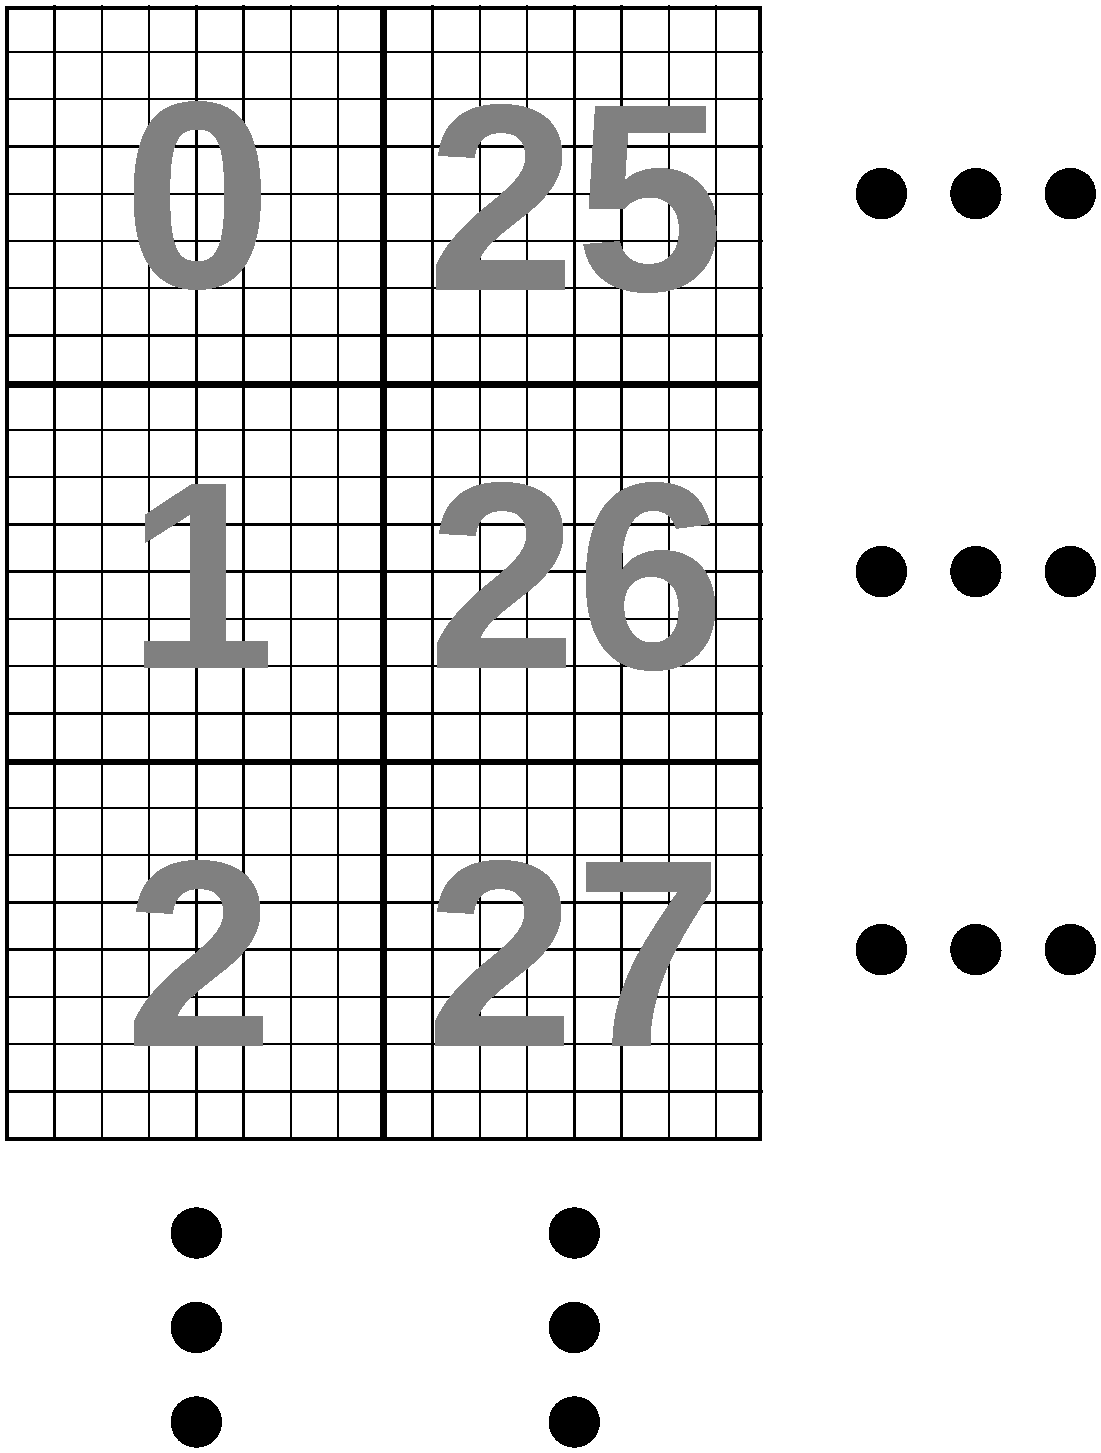
\includegraphics[width=0.7\textwidth]{images/illustrations/char-tile-grid-vertical-numbered}
\end{center}

Door de tekens zo in verticale kolommen te rangschikken, levert een verticale verplaatsing van één pixel telkens een constante toename van 8 bytes op, zoals hieronder wordt weergegeven:

\begin{center}
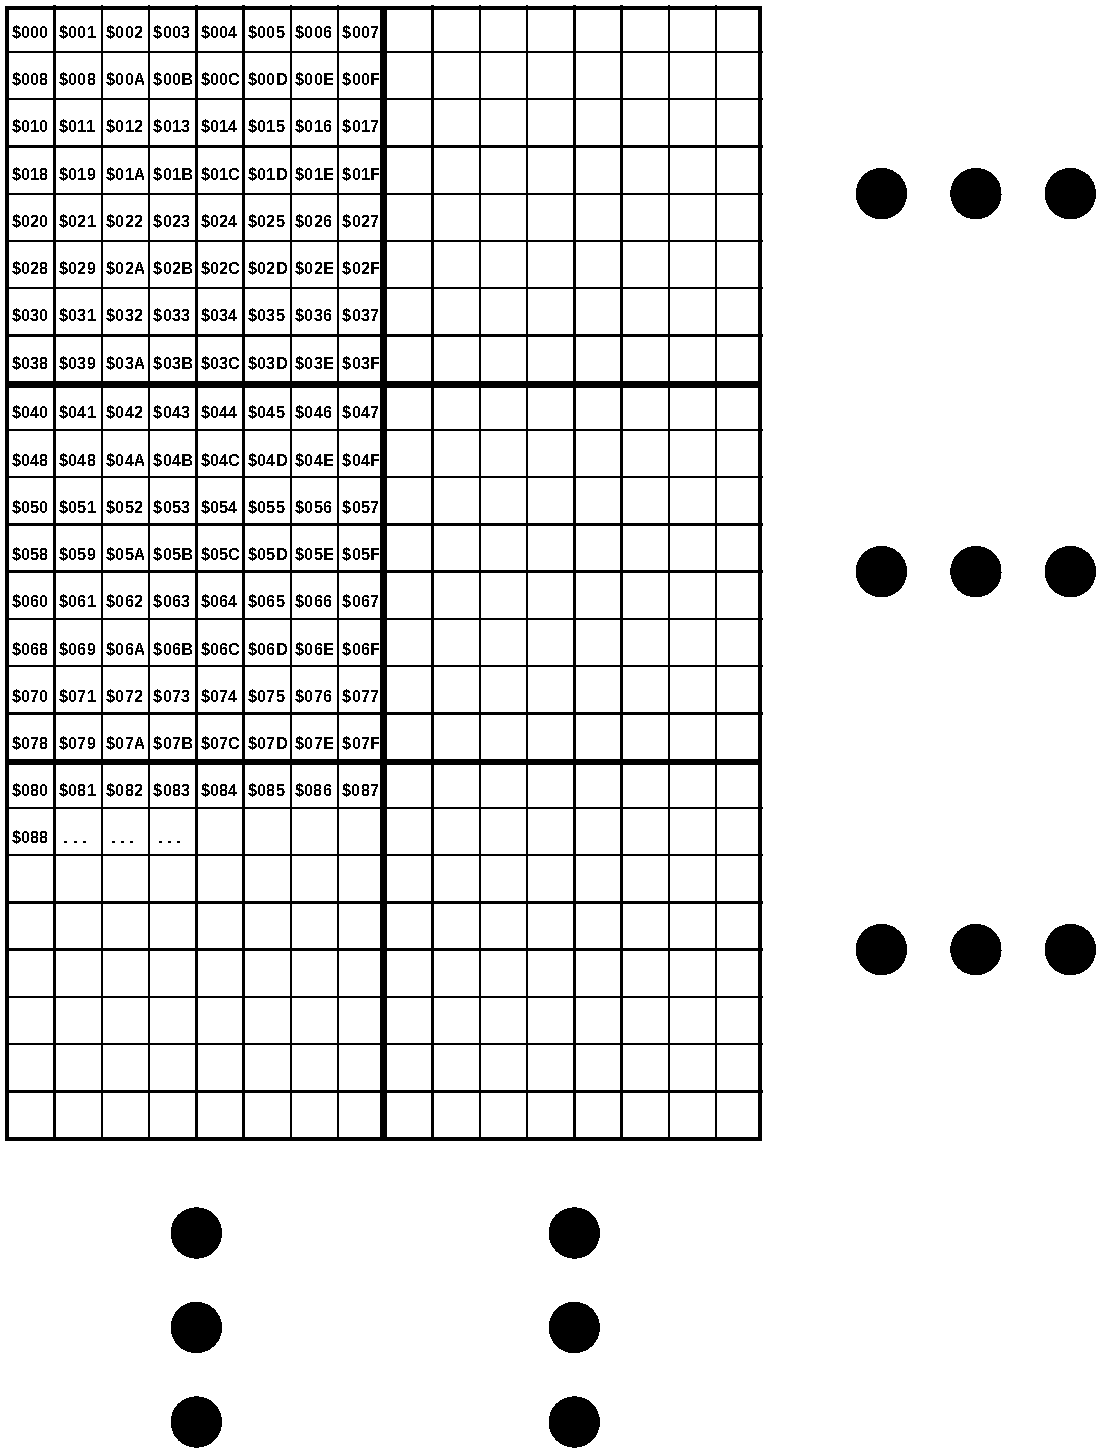
\includegraphics[width=0.7\textwidth]{images/illustrations/char-tile-grid-vertical-addressed}
\end{center}


De skipwaarden voor bron en bestemming maken het ook mogelijk de schaalfactoren in te stellen. Een skipwaarde van \$0100 komt overeen met een verplaatsing van \$01.00 pixel. Wilt u de verticaal gestapelde FCM-indeling gebruiken als doel voor het kopiëren van verticale textuurlijnen, dan moet de bestemmingsskipwaarde \$0800 zijn, d.w.z. 8.0 bytes per pixel. Daarmee wordt een verticale lijn textuurgegevens zonder schaling gekopieerd. Door de bronverplaatsing lager dan \$0100 in te stellen, worden sommige pixels herhaald, waardoor de textuur effectief wordt ingezoomd; stelt u de bronverplaatsing boven \$0100 in, dan worden sommige pixels overgeslagen, waardoor de textuur effectief wordt uitgezoomd. De bestemmingsverplaatsing hoeft gewoonlijk niet te worden aangepast. Let op: de textuurgegevens moeten zo worden opgeslagen dat elke verticale strook aaneengesloten staat, opdat deze modus kan worden gebruikt.

Voor het tekenen van lijnen moet de DMA-controller de schermindeling kennen. Hij moet in het bijzonder weten welk getal moet worden opgeteld bij het adres van de meest rechtse pixel in een kolom FCM-tekens om het adres te berekenen van de pixel die onmiddellijk rechts daarvan verschijnt. Evenzo moet hij weten hoeveel er moet worden opgeteld bij het adres van de onderste pixel in een rij FCM-tekens om het adres te berekenen van de pixel die onmiddellijk onder die pixel verschijnt. Dit biedt flexibele mogelijkheden voor de schermindeling en willekeurige schermafmetingen. U moet daarna ook de helling van de lijn opgeven, of de lijn de X-as of de Y-as als hoofdas heeft en of de helling positief of negatief is.

Het bestand {\tt test\_290.c} in de repository \url{https://github.com/mega65/mega65-tools} bevat een voorbeeld van het gebruik van deze voorzieningen om hardware-versnelde lijntekening te implementeren. Deze aanpak is {\em zeer} snel, want de lijnen worden getekend met de volledige DMA-vulsnelheid, d.w.z. ongeveer 40.5 miljoen pixels per seconde.

\section{Inline-DMA-lijsten}
\index{DMA!Inline-DMA-lijsten}
\index{Inline-DMA-lijsten}

Gewoonlijk moet u een apart geheugengebied inrichten dat de DMA-lijst bevat en vervolgens het adres van dat gebied in de DMA-adresregisters op \$D70x laden. Omdat de DMA-controller van de MEGA65 deel uitmaakt van de CPU, ondersteunt deze bovendien een uiterst handige extra modus: de inline-DMA-lijstmodus.

Deze modus werkt zoals de Enhanced-DMA-modus, met dit verschil dat de DMA-lijst wordt gelezen vanaf de huidige waarde van het Program Counter (PC)-register. Om deze modus te gebruiken, schrijft u een willekeurige waarde naar \$D707. Hiermee start u onmiddellijk een DMA-taak, waarvan de lijst staat in de bytes die direct volgen op de instructie die naar \$D707 schrijft.

De DMA-lijst kan uit één enkele taak bestaan of, zoals bij elke andere DMA-taak, uit meerdere gekoppelde taken. Het echte kunststuk is dat de programmateller wordt gezet op het eerstvolgende adres na het einde van de DMA-lijst en dat de DMA-lijst wordt gelezen uit de huidige geheugenindeling van de CPU. Dit betekent dat u code met DMA-lijsten vanuit elke geheugenbank kunt uitvoeren, zonder dat u hoeft na te gaan in welke bank die code staat.

Het volgende codevoorbeeld wist bijvoorbeeld het scherm in de C65-modus en laat de rand daarna eindeloos flikkeren:

\begin{asmcodesmall}
  STA $D707
  .byte $00   ; end of job options
  .byte $03   ; fill
  .word 2000  ; count
  .word $0020 ; value
  .byte $00   ; src bank
  .word $0800 ; dst
  .byte $00   ; dst bank
  .byte $00   ; cmd hi
  .word $0000 ; modulo / ignored
foo:
  INC $D020
  JMP foo
\end{asmcodesmall}

\section{Audio-DMA}
\index{Digitale audio}
\index{DMA-audio}
\index{Amiga\texttrademark{}-stijl audio}
\index{MOD-stijl audio}
De MEGA65 beschikt over vier kanalen voor DMA-aangestuurde geluidsweergave, die in plaats van de directe digitale audioregisters op \$D6F8-\$D6FB gebruikt kunnen worden. U moet dus kiezen welke van deze twee bronnen u aan de audio-crossbar-mixer wilt toevoeren. Die keuze wordt gemaakt via het AUDEN-signaal (bit 7 van \$D711), dat tegelijkertijd de audio-DMA-functie in de processor inschakelt en de audio-crossbar-mixer opdraagt de audio van deze bron te gebruiken in plaats van de digitale audioregisters op \$D6F8-\$D6FB. Indien u naast de audio-DMA-kanalen geen ander geluid wenst, kan de audio-crossbar-mixer worden omzeild en kan de DMA-audio op vol volume worden afgespeeld door het NOMIX-signaal te zetten (bit 4 van \$D711). De omzeiling geldt alleen voor de PWM-audio-uitgangen (de 3,5mm-audioaansluiting op R3 en oudere borden): op die uitgangen is er geen geluid van de SID's, FM, microfoons of andere bronnen beschikbaar. HDMI-audio, en de audio-DAC op R4 en nieuwere borden, dragen altijd de uitvoer van de audio-crossbar-mixer. Alle overige bits van \$D711 moeten gewoonlijk nul blijven; schrijf dus \$80 naar \$D711 om audio-DMA in te schakelen.

Twee kanalen vormen het linker digitale audiokanaal en de twee andere het rechter digitale audiokanaal. Deze linker- en rechterkanalen worden vervolgens aan de audio-crossbar-mixer van de MEGA65 toegevoerd.

Omdat de DMA-controller deel uitmaakt van de processor van de MEGA65 en de MEGA65 geen gereserveerde busesleuven heeft voor multimedia-bewerkingen, gebruikt de MEGA65 ongebruikte CPU-cycli om DMA op de achtergrond uit te voeren. Hiervoor moet de CPU van de MEGA65 in de modus ``full speed'' staan, d.w.z. op ongeveer 40 MHz. In deze modus treedt bij het lezen van een operand uit het geheugen telkens een wachtcyclus op. Elke instructie die een byte uit het geheugen laadt, creëert daardoor één impliciete audio-DMA-sleuf. In de praktijk is dit zelden een probleem, behalve wanneer de processor in een zeer strakke lus wacht. Om ervoor te zorgen dat de audio op de achtergrond blijft spelen, moeten dergelijke lussen een leesinstructie bevatten, zoals:

\begin{asmcodesmall}
  ; Ensure loop has at least one idle cycle for
  ; audio DMA
loop:
  LDA $1234
  JMP loop
\end{asmcodesmall}

Elk van de vier DMA-kanalen wordt geconfigureerd met een blok van 16 registers op respectievelijk \$D720, \$D730, \$D740 en \$D750. Wij lichten de registers van het eerste kanaal, kanaal 0, toe op \$D720 -- \$D72F.

\subsection{Adresbeheer voor samples}

Om een audiosample af te spelen, moet u eerst het startadres van het sample opgeven. Dit is een 24-bits adres dat in het hoofd-chipgeheugen van de MEGA65 moet liggen. U schrijft het adres daartoe in \$D72A -- \$D72C. Dat is het adres van de eerste samplewaarde die wordt afgespeeld. Vervolgens moet u het eindadres van het sample opgeven in \$D727 -- \$D728. Let echter op: dit is slechts 16 bits. Dat komt doordat de MEGA65 bij de controle of het einde van een sample is bereikt, alleen de onderste 16 bits van het adres vergelijkt. In de praktijk betekent dit dat samples niet groter dan 64 KB kunnen zijn. Bevat het sample een gedeelte dat herhaald moet worden, dan moet het startadres van dat herhalende gedeelte in \$D721 -- \$D723 worden geladen en moet de CH0LOOP-bit worden gezet (bit 6 van \$D720).

U kunt op elk moment het huidige sampleadres bepalen door de registers op \$D72A -- \$D72C te lezen. Let echter op: deze registers worden niet vergrendeld, zodat de waarden tijdens het lezen kunnen worden bijgewerkt, tenzij u het kanaal eerst stopt door het CH0EN-signaal te wissen.

\subsection{Afspeelfrequentie en volume van samples}

De MEGA65 regelt de afspeelsnelheid van audio-DMA-samples met een 24-bits teller. Telkens wanneer de 24-bits teller overloopt, wordt de volgende samplewaarde opgevraagd. De samplesnelheid stelt u in door de waarde te kiezen die elke CPU-cyclus aan deze teller wordt toegevoegd. Een waarde van \$FFFFFF levert derhalve een samplerate van bijna 40.5 MHz op. In de praktijk zijn samplerates boven enkele megahertz echter niet mogelijk, omdat daarvoor onvoldoende ongebruikte CPU-cycli beschikbaar zijn en er anders vervormd geluid ontstaat. Ook onder die grens moet u ervoor zorgen dat de ongebruikte cycli voldoende vaak en voldoende verspreid door de instructiestroom van de processor voorkomen, om vervorming te vermijden. Bij typische samplerates onder 16 kHz en het gebruik van 8-bits samples zijn deze effecten voor normale instructiestromen doorgaans verwaarloosbaar, zodat voor normaal audio-afspelen gewoonlijk geen speciale maatregelen nodig zijn.

Aan de andere kant van de schaal zijn samplefrequenties van slechts 40.5 MHz/$2^{24}$= 2.4 samples per seconde mogelijk. Dat is laag genoeg voor zelfs de meest veeleisende infrageluidstoepassingen.

Het volume wordt geregeld door \$D729 in te stellen. Het maximale volume wordt bereikt met de waarde \$FF, terwijl een waarde van \$00 het kanaal volledig dempt. De eerste twee audiokanalen worden normaal gesproken aan de linkerzijde toegewezen en de tweede twee aan de rechterzijde. De MEGA65 beschikt echter over afzonderlijke volumeregelaars voor de tegenoverliggende kanalen. Om audio-DMA-kanaal 0 bijvoorbeeld op vol volume aan zowel de linker- als de rechterkant van de audio-uitgang af te spelen, stelt u zowel \$D729 als \$D71C in op \$FF. Dit maakt het pannen van de vier audio-DMA-kanalen mogelijk.

Zowel de frequentie als het volume kunnen tijdens het afspelen van een sample vrij worden aangepast om verschillende effecten te verkrijgen.

\subsection{Zuivere sinusgolf}

Wanneer het nodig is een stabiele sinusgolf te produceren, met name bij hogere frequenties, voorziet een speciale modus hierin. Door het CH0SINE-signaal te zetten, speelt het audiokanaal een sinusgolfpatroon van 32 bytes met 16-bits samples af. De sample-adressen moeten nog steeds worden ingesteld, alsof de sinusgolftabel zich in de onderste 64 bytes van het geheugen bevindt; de normale adresgeneratielogica wordt namelijk ook in deze modus gebruikt. In deze modus worden geen audio-DMA-fetches uitgevoerd, zodat alle vervormingsbronnen worden vermeden die het gevolg zijn van de onregelmatige spreiding van inactieve cycli in de instructiestroom van de processor.

Dit kan worden gebruikt om sinusgolven te produceren in zowel het hoorbare bereik als ver daarboven in het ultrasone bereik, bij frequenties die 60000 Hz overschrijden, mits de MEGA65 is aangesloten op een geschikte luidsprekeropstelling.

\subsection{Regeling van het afspelen van samples}

Om een kanaal een sample te laten afspelen, zet u het CH0EN-signaal (\$D720 bit 7). Het sample wordt afgespeeld tot het zijn einde bereikt, tenzij het CH0LOOP-signaal eveneens is gezet. Wanneer een sample klaar is met afspelen, wordt de CH0STP-vlag gezet. Het audio-DMA-subsysteem kan op dit moment geen interrupts genereren.

Anders dan de Amiga\texttrademark{} biedt het audio-DMA-systeem van de MEGA65 ondersteuning voor zowel 8- als 16-bits samples. Het ondersteunt ook samengepakte 4-bits samples, waarbij van elk sample-byte de lagere of de hogere nibble wordt afgespeeld. Hierdoor kunnen twee afzonderlijke samples hetzelfde byte bezetten, waarmee de benodigde opslagruimte voor twee samples van gelijke lengte effectief wordt gehalveerd.

\section{F018 ``DMAgic'' DMA-controller}

\setlength{\tabcolsep}{0pt}
\begin{longtable}{|C{12.5mm}|C{12.5mm}|C{12.5mm}|C{12.5mm}|C{12.5mm}|C{12.5mm}|C{12.5mm}|C{12.5mm}|C{12.5mm}|C{12.5mm}|}
\hline
{\bf{HEX}} & {\bf{DEC}} & {\bf{DB7}} & {\bf{DB6}} & {\bf{DB5}} & {\bf{DB4}} & {\bf{DB3}} & {\bf{DB2}} & {\bf{DB1}} & {\bf{DB0}} \\
\hline
\endfirsthead
\multicolumn{3}{l@{}}{\ldots vervolgd}\\
\hline
{\bf{HEX}} & {\bf{DEC}} & {\bf{DB7}} & {\bf{DB6}} & {\bf{DB5}} & {\bf{DB4}} & {\bf{DB3}} & {\bf{DB2}} & {\bf{DB1}} & {\bf{DB0}} \\
\endhead
\multicolumn{3}{l@{}}{vervolgd \ldots}\\
\endfoot
\hline
\endlastfoot
\footnotesize  D700\index{Registers!\$D700} \index{Registers!55040} & \footnotesize 55040 & \multicolumn{8}{c|}{\footnotesize ADDRLSBTRIG\index{Registers!ADDRLSBTRIG}}\\
\hline
\footnotesize  D701\index{Registers!\$D701} \index{Registers!55041} & \footnotesize 55041 & \multicolumn{8}{c|}{\footnotesize ADDRMSB\index{Registers!ADDRMSB}}\\
\hline
\footnotesize  D702\index{Registers!\$D702} \index{Registers!55042} & \footnotesize 55042 & \footnotesize WITHIO & \multicolumn{7}{c|}{\footnotesize ADDRBANK\index{Registers!ADDRBANK}}\\
\hline
\end{longtable}
\begin{itemize}
\item{\bf{ADDRBANK}\index{Registers!ADDRBANK}} Adresbank van de DMA-lijst (bits 16 - 22). Schrijven wist \$D704.
\item{\bf{ADDRLSBTRIG}\index{Registers!ADDRLSBTRIG}} DMAgic-LSB van het adres van de DMA-lijst (bits 0 - 7); start DMA wanneer erin wordt geschreven
\item{\bf{ADDRMSB}\index{Registers!ADDRMSB}} Hoge byte van het adres van de DMA-lijst (bits 8 - 15)
\item{\bf{WITHIO}\index{Registers!WITHIO}} DMA-withio-vlag (onbenut)
\end{itemize}


\section{Uitbreidingen van de MEGA65-DMA-controller}

\setlength{\tabcolsep}{0pt}
\begin{longtable}{|C{12.5mm}|C{12.5mm}|C{12.5mm}|C{12.5mm}|C{12.5mm}|C{12.5mm}|C{12.5mm}|C{12.5mm}|C{12.5mm}|C{12.5mm}|}
\hline
{\bf{HEX}} & {\bf{DEC}} & {\bf{DB7}} & {\bf{DB6}} & {\bf{DB5}} & {\bf{DB4}} & {\bf{DB3}} & {\bf{DB2}} & {\bf{DB1}} & {\bf{DB0}} \\
\hline
\endfirsthead
\multicolumn{3}{l@{}}{\ldots vervolgd}\\
\hline
{\bf{HEX}} & {\bf{DEC}} & {\bf{DB7}} & {\bf{DB6}} & {\bf{DB5}} & {\bf{DB4}} & {\bf{DB3}} & {\bf{DB2}} & {\bf{DB1}} & {\bf{DB0}} \\
\endhead
\multicolumn{3}{l@{}}{vervolgd \ldots}\\
\endfoot
\hline
\endlastfoot
\footnotesize  D703\index{Registers!\$D703} \index{Registers!55043} & \footnotesize 55043 & \multicolumn{6}{c|}{\footnotesize --}& \footnotesize NOMBWRAP & \footnotesize EN018B \\
\hline
\footnotesize  D704\index{Registers!\$D704} \index{Registers!55044} & \footnotesize 55044 & \multicolumn{8}{c|}{\footnotesize ADDRMB\index{Registers!ADDRMB}}\\
\hline
\footnotesize  D705\index{Registers!\$D705} \index{Registers!55045} & \footnotesize 55045 & \multicolumn{8}{c|}{\footnotesize ETRIG\index{Registers!ETRIG}}\\
\hline
\footnotesize  D706\index{Registers!\$D706} \index{Registers!55046} & \footnotesize 55046 & \multicolumn{8}{c|}{\footnotesize ETRIGMAPD\index{Registers!ETRIGMAPD}}\\
\hline
\footnotesize  D707\index{Registers!\$D707} \index{Registers!55047} & \footnotesize 55047 & \multicolumn{8}{c|}{\footnotesize ETRIGINLINE\index{Registers!ETRIGINLINE}}\\
\hline
\footnotesize  D70E\index{Registers!\$D70E} \index{Registers!55054} & \footnotesize 55054 & \multicolumn{8}{c|}{\footnotesize ADDRLSB\index{Registers!ADDRLSB}}\\
\hline
\footnotesize  D711\index{Registers!\$D711} \index{Registers!55057} & \footnotesize 55057 & \footnotesize AUDEN & \footnotesize BLKD & \footnotesize AUD\-WRBLK & \footnotesize NOMIX & \footnotesize -- & \multicolumn{3}{c|}{\footnotesize AUD\-BLKTO\index{Registers!AUDBLKTO}}\\
\hline
\footnotesize  D712\index{Registers!\$D712} \index{Registers!55058} & \footnotesize 55058 & \footnotesize DBG\-LFTCLP & \footnotesize DBG\-RGTCLP & \multicolumn{4}{c|}{\footnotesize --}& \footnotesize CHANSWAP & \footnotesize -- \\
\hline
\footnotesize  D713\index{Registers!\$D713} \index{Registers!55059} & \footnotesize 55059 & \footnotesize IRQ\-CH0FLG & \footnotesize IRQ\-CH1FLG & \footnotesize IRQ\-CH2FLG & \footnotesize IRQ\-CH3FLG & \footnotesize IRQ\-CH0ENA & \footnotesize IRQ\-CH1ENA & \footnotesize IRQ\-CH2ENA & \footnotesize IRQ\-CH3ENA \\
\hline
\footnotesize  D714\index{Registers!\$D714} \index{Registers!55060} & \footnotesize 55060 & \multicolumn{8}{c|}{\footnotesize IRQ\-CH0OFFS\index{Registers!CHXOFFS}}\\
\hline
\footnotesize  D715\index{Registers!\$D715} \index{Registers!55061} & \footnotesize 55061 & \multicolumn{8}{c|}{\footnotesize IRQ\-CH1OFFS\index{Registers!IRQCH1OFFS}}\\
\hline
\footnotesize  D716\index{Registers!\$D716} \index{Registers!55062} & \footnotesize 55062 & \multicolumn{8}{c|}{\footnotesize IRQ\-CH2OFFS\index{Registers!IRQCH2OFFS}}\\
\hline
\footnotesize  D717\index{Registers!\$D717} \index{Registers!55063} & \footnotesize 55063 & \multicolumn{8}{c|}{\footnotesize IRQ\-CH3OFFS\index{Registers!IRQCH3OFFS}}\\
\hline
\footnotesize  D71C\index{Registers!\$D71C} \index{Registers!55068} & \footnotesize 55068 & \multicolumn{8}{c|}{\footnotesize CH0RVOL\index{Registers!CH0RVOL}}\\
\hline
\footnotesize  D71D\index{Registers!\$D71D} \index{Registers!55069} & \footnotesize 55069 & \multicolumn{8}{c|}{\footnotesize CH1RVOL\index{Registers!CH1RVOL}}\\
\hline
\footnotesize  D71E\index{Registers!\$D71E} \index{Registers!55070} & \footnotesize 55070 & \multicolumn{8}{c|}{\footnotesize CH2LVOL\index{Registers!CH2LVOL}}\\
\hline
\footnotesize  D71F\index{Registers!\$D71F} \index{Registers!55071} & \footnotesize 55071 & \multicolumn{8}{c|}{\footnotesize CH3LVOL\index{Registers!CH3LVOL}}\\
\hline
\footnotesize  D720\index{Registers!\$D720} \index{Registers!55072} & \footnotesize 55072 & \footnotesize CH0\-EN & \footnotesize CH0\-LOOP & \footnotesize CH0\-SGN & \footnotesize CH0\-SINE & \footnotesize CH0\-STP & \footnotesize -- & \multicolumn{2}{c|}{\footnotesize CH0\-SBITS\index{Registers!CHXSBITS}}\\
\hline
\footnotesize  D721\index{Registers!\$D721} \index{Registers!55073} & \footnotesize 55073 & \multicolumn{8}{c|}{\footnotesize CH0BADDRLSB\index{Registers!CHXBADDRLSB}}\\
\hline
\footnotesize  D722\index{Registers!\$D722} \index{Registers!55074} & \footnotesize 55074 & \multicolumn{8}{c|}{\footnotesize CH0BADDRMSB\index{Registers!CHXBADDRMSB}}\\
\hline
\footnotesize  D723\index{Registers!\$D723} \index{Registers!55075} & \footnotesize 55075 & \multicolumn{8}{c|}{\footnotesize CH0BADDRBNK\index{Registers!CHXBADDRBNK}}\\
\hline
\footnotesize  D724\index{Registers!\$D724} \index{Registers!55076} & \footnotesize 55076 & \multicolumn{8}{c|}{\footnotesize CH0FREQ0\index{Registers!CHXFREQ0}}\\
\hline
\footnotesize  D725\index{Registers!\$D725} \index{Registers!55077} & \footnotesize 55077 & \multicolumn{8}{c|}{\footnotesize CH0FREQ1\index{Registers!CHXFREQ1}}\\
\hline
\footnotesize  D726\index{Registers!\$D726} \index{Registers!55078} & \footnotesize 55078 & \multicolumn{8}{c|}{\footnotesize CH0FREQ2\index{Registers!CHXFREQ2}}\\
\hline
\footnotesize  D727\index{Registers!\$D727} \index{Registers!55079} & \footnotesize 55079 & \multicolumn{8}{c|}{\footnotesize CH0TADDRLSB\index{Registers!CHXTADDRL}}\\
\hline
\footnotesize  D728\index{Registers!\$D728} \index{Registers!55080} & \footnotesize 55080 & \multicolumn{8}{c|}{\footnotesize CH0TADDRMSB\index{Registers!CHXTADDRM}}\\
\hline
\footnotesize  D729\index{Registers!\$D729} \index{Registers!55081} & \footnotesize 55081 & \multicolumn{8}{c|}{\footnotesize CH0VOLUME\index{Registers!CHXVOLUME}}\\
\hline
\footnotesize  D72A\index{Registers!\$D72A} \index{Registers!55082} & \footnotesize 55082 & \multicolumn{8}{c|}{\footnotesize CH0CURADDRLSB\index{Registers!CHXCURADDRLSB}}\\
\hline
\footnotesize  D72B\index{Registers!\$D72B} \index{Registers!55083} & \footnotesize 55083 & \multicolumn{8}{c|}{\footnotesize CH0CURADDRMSB\index{Registers!CHXCURADDRMSB}}\\
\hline
\footnotesize  D72C\index{Registers!\$D72C} \index{Registers!55084} & \footnotesize 55084 & \multicolumn{8}{c|}{\footnotesize CH0CURADDRBNK\index{Registers!CHXCURADDRBNK}}\\
\hline
\footnotesize  D72D\index{Registers!\$D72D} \index{Registers!55085} & \footnotesize 55085 & \multicolumn{8}{c|}{\footnotesize CH0TMGCNT0\index{Registers!CHXTMGCNT0}}\\
\hline
\footnotesize  D72E\index{Registers!\$D72E} \index{Registers!55086} & \footnotesize 55086 & \multicolumn{8}{c|}{\footnotesize CH0TMGCNT1\index{Registers!CHXTMGCNT1}}\\
\hline
\footnotesize  D72F\index{Registers!\$D72F} \index{Registers!55087} & \footnotesize 55087 & \multicolumn{8}{c|}{\footnotesize CH0TMGCNT2\index{Registers!CHXTMGCNT2}}\\
\hline
\footnotesize  D730\index{Registers!\$D730} \index{Registers!55088} & \footnotesize 55088 & \footnotesize CH1\-EN & \footnotesize CH1\-LOOP & \footnotesize CH1\-SGN & \footnotesize CH1\-SINE & \footnotesize CH1\-STP & \footnotesize -- & \multicolumn{2}{c|}{\footnotesize CH1\-SBITS\index{Registers!CH1SBITS}}\\
\hline
\footnotesize  D731\index{Registers!\$D731} \index{Registers!55089} & \footnotesize 55089 & \multicolumn{8}{c|}{\footnotesize CH1BADDRLSB\index{Registers!CH1BADDRLSB}}\\
\hline
\footnotesize  D732\index{Registers!\$D732} \index{Registers!55090} & \footnotesize 55090 & \multicolumn{8}{c|}{\footnotesize CH1BADDRMSB\index{Registers!CH1BADDRMSB}}\\
\hline
\footnotesize  D733\index{Registers!\$D733} \index{Registers!55091} & \footnotesize 55091 & \multicolumn{8}{c|}{\footnotesize CH1BADDRBNK\index{Registers!CH1BADDRBNK}}\\
\hline
\footnotesize  D734\index{Registers!\$D734} \index{Registers!55092} & \footnotesize 55092 & \multicolumn{8}{c|}{\footnotesize CH1FREQ0\index{Registers!CH1FREQ0}}\\
\hline
\footnotesize  D735\index{Registers!\$D735} \index{Registers!55093} & \footnotesize 55093 & \multicolumn{8}{c|}{\footnotesize CH1FREQ1\index{Registers!CH1FREQ1}}\\
\hline
\footnotesize  D736\index{Registers!\$D736} \index{Registers!55094} & \footnotesize 55094 & \multicolumn{8}{c|}{\footnotesize CH1FREQ2\index{Registers!CH1FREQ2}}\\
\hline
\footnotesize  D737\index{Registers!\$D737} \index{Registers!55095} & \footnotesize 55095 & \multicolumn{8}{c|}{\footnotesize CH1TADDRLSB\index{Registers!CH1TADDRLSB}}\\
\hline
\footnotesize  D738\index{Registers!\$D738} \index{Registers!55096} & \footnotesize 55096 & \multicolumn{8}{c|}{\footnotesize CH1TADDRMSB\index{Registers!CH1TADDRMSB}}\\
\hline
\footnotesize  D739\index{Registers!\$D739} \index{Registers!55097} & \footnotesize 55097 & \multicolumn{8}{c|}{\footnotesize CH1VOLUME\index{Registers!CH1VOLUME}}\\
\hline
\footnotesize  D73A\index{Registers!\$D73A} \index{Registers!55098} & \footnotesize 55098 & \multicolumn{8}{c|}{\footnotesize CH1CURADDRLSB\index{Registers!CH1CURADDRLSB}}\\
\hline
\footnotesize  D73B\index{Registers!\$D73B} \index{Registers!55099} & \footnotesize 55099 & \multicolumn{8}{c|}{\footnotesize CH1CURADDRMSB\index{Registers!CH1CURADDRMSB}}\\
\hline
\footnotesize  D73C\index{Registers!\$D73C} \index{Registers!55100} & \footnotesize 55100 & \multicolumn{8}{c|}{\footnotesize CH1CURADDRBNK\index{Registers!CH1CURADDRBNK}}\\
\hline
\footnotesize  D73D\index{Registers!\$D73D} \index{Registers!55101} & \footnotesize 55101 & \multicolumn{8}{c|}{\footnotesize CH1TMGCNT0\index{Registers!CH1TMGCNT0}}\\
\hline
\footnotesize  D73E\index{Registers!\$D73E} \index{Registers!55102} & \footnotesize 55102 & \multicolumn{8}{c|}{\footnotesize CH1TMGCNT1\index{Registers!CH1TMGCNT1}}\\
\hline
\footnotesize  D73F\index{Registers!\$D73F} \index{Registers!55103} & \footnotesize 55103 & \multicolumn{8}{c|}{\footnotesize CH1TMGCNT2\index{Registers!CH1TMGCNT2}}\\
\hline
\footnotesize  D740\index{Registers!\$D740} \index{Registers!55104} & \footnotesize 55104 & \footnotesize CH2\-EN & \footnotesize CH2\-LOOP & \footnotesize CH2\-SGN & \footnotesize CH2\-SINE & \footnotesize CH2\-STP & \footnotesize -- & \multicolumn{2}{c|}{\footnotesize CH2\-SBITS\index{Registers!CH2SBITS}}\\
\hline
\footnotesize  D741\index{Registers!\$D741} \index{Registers!55105} & \footnotesize 55105 & \multicolumn{8}{c|}{\footnotesize CH2BADDRLSB\index{Registers!CH2BADDRLSB}}\\
\hline
\footnotesize  D742\index{Registers!\$D742} \index{Registers!55106} & \footnotesize 55106 & \multicolumn{8}{c|}{\footnotesize CH2BADDRMSB\index{Registers!CH2BADDRMSB}}\\
\hline
\footnotesize  D743\index{Registers!\$D743} \index{Registers!55107} & \footnotesize 55107 & \multicolumn{8}{c|}{\footnotesize CH2BADDRBNK\index{Registers!CH2BADDRBNK}}\\
\hline
\footnotesize  D744\index{Registers!\$D744} \index{Registers!55108} & \footnotesize 55108 & \multicolumn{8}{c|}{\footnotesize CH2FREQ0\index{Registers!CH2FREQ0}}\\
\hline
\footnotesize  D745\index{Registers!\$D745} \index{Registers!55109} & \footnotesize 55109 & \multicolumn{8}{c|}{\footnotesize CH2FREQ1\index{Registers!CH2FREQ1}}\\
\hline
\footnotesize  D746\index{Registers!\$D746} \index{Registers!55110} & \footnotesize 55110 & \multicolumn{8}{c|}{\footnotesize CH2FREQ2\index{Registers!CH2FREQ2}}\\
\hline
\footnotesize  D747\index{Registers!\$D747} \index{Registers!55111} & \footnotesize 55111 & \multicolumn{8}{c|}{\footnotesize CH2TADDRLSB\index{Registers!CH2TADDRLSB}}\\
\hline
\footnotesize  D748\index{Registers!\$D748} \index{Registers!55112} & \footnotesize 55112 & \multicolumn{8}{c|}{\footnotesize CH2TADDRMSB\index{Registers!CH2TADDRMSB}}\\
\hline
\footnotesize  D749\index{Registers!\$D749} \index{Registers!55113} & \footnotesize 55113 & \multicolumn{8}{c|}{\footnotesize CH2VOLUME\index{Registers!CH2VOLUME}}\\
\hline
\footnotesize  D74A\index{Registers!\$D74A} \index{Registers!55114} & \footnotesize 55114 & \multicolumn{8}{c|}{\footnotesize CH2CURADDRLSB\index{Registers!CH2CURADDRLSB}}\\
\hline
\footnotesize  D74B\index{Registers!\$D74B} \index{Registers!55115} & \footnotesize 55115 & \multicolumn{8}{c|}{\footnotesize CH2CURADDRMSB\index{Registers!CH2CURADDRMSB}}\\
\hline
\footnotesize  D74C\index{Registers!\$D74C} \index{Registers!55116} & \footnotesize 55116 & \multicolumn{8}{c|}{\footnotesize CH2CURADDRBNK\index{Registers!CH2CURADDRBNK}}\\
\hline
\footnotesize  D74D\index{Registers!\$D74D} \index{Registers!55117} & \footnotesize 55117 & \multicolumn{8}{c|}{\footnotesize CH2TMGCNT0\index{Registers!CH2TMGCNT0}}\\
\hline
\footnotesize  D74E\index{Registers!\$D74E} \index{Registers!55118} & \footnotesize 55118 & \multicolumn{8}{c|}{\footnotesize CH2TMGCNT1\index{Registers!CH2TMGCNT1}}\\
\hline
\footnotesize  D74F\index{Registers!\$D74F} \index{Registers!55119} & \footnotesize 55119 & \multicolumn{8}{c|}{\footnotesize CH2TMGCNT2\index{Registers!CH2TMGCNT2}}\\
\hline
\footnotesize  D750\index{Registers!\$D750} \index{Registers!55120} & \footnotesize 55120 & \footnotesize CH3\-EN & \footnotesize CH3\-LOOP & \footnotesize CH3\-SGN & \footnotesize CH3\-SINE & \footnotesize CH3\-STP & \footnotesize -- & \multicolumn{2}{c|}{\footnotesize CH3\-SBITS\index{Registers!CH3SBITS}}\\
\hline
\footnotesize  D751\index{Registers!\$D751} \index{Registers!55121} & \footnotesize 55121 & \multicolumn{8}{c|}{\footnotesize CH3BADDRLSB\index{Registers!CH3BADDRLSB}}\\
\hline
\footnotesize  D752\index{Registers!\$D752} \index{Registers!55122} & \footnotesize 55122 & \multicolumn{8}{c|}{\footnotesize CH3BADDRMSB\index{Registers!CH3BADDRMSB}}\\
\hline
\footnotesize  D753\index{Registers!\$D753} \index{Registers!55123} & \footnotesize 55123 & \multicolumn{8}{c|}{\footnotesize CH3BADDRBNK\index{Registers!CH3BADDRBNK}}\\
\hline
\footnotesize  D754\index{Registers!\$D754} \index{Registers!55124} & \footnotesize 55124 & \multicolumn{8}{c|}{\footnotesize CH3FREQ0\index{Registers!CH3FREQ0}}\\
\hline
\footnotesize  D755\index{Registers!\$D755} \index{Registers!55125} & \footnotesize 55125 & \multicolumn{8}{c|}{\footnotesize CH3FREQ1\index{Registers!CH3FREQ1}}\\
\hline
\footnotesize  D756\index{Registers!\$D756} \index{Registers!55126} & \footnotesize 55126 & \multicolumn{8}{c|}{\footnotesize CH3FREQ2\index{Registers!CH3FREQ2}}\\
\hline
\footnotesize  D757\index{Registers!\$D757} \index{Registers!55127} & \footnotesize 55127 & \multicolumn{8}{c|}{\footnotesize CH3TADDRLSB\index{Registers!CH3TADDRLSB}}\\
\hline
\footnotesize  D758\index{Registers!\$D758} \index{Registers!55128} & \footnotesize 55128 & \multicolumn{8}{c|}{\footnotesize CH3TADDRMSB\index{Registers!CH3TADDRMSB}}\\
\hline
\footnotesize  D759\index{Registers!\$D759} \index{Registers!55129} & \footnotesize 55129 & \multicolumn{8}{c|}{\footnotesize CH3VOLUME\index{Registers!CH3VOLUME}}\\
\hline
\footnotesize  D75A\index{Registers!\$D75A} \index{Registers!55130} & \footnotesize 55130 & \multicolumn{8}{c|}{\footnotesize CH3CURADDRLSB\index{Registers!CH3CURADDRLSB}}\\
\hline
\footnotesize  D75B\index{Registers!\$D75B} \index{Registers!55131} & \footnotesize 55131 & \multicolumn{8}{c|}{\footnotesize CH3CURADDRMSB\index{Registers!CH3CURADDRMSB}}\\
\hline
\footnotesize  D75C\index{Registers!\$D75C} \index{Registers!55132} & \footnotesize 55132 & \multicolumn{8}{c|}{\footnotesize CH3CURADDRBNK\index{Registers!CH3CURADDRBNK}}\\
\hline
\footnotesize  D75D\index{Registers!\$D75D} \index{Registers!55133} & \footnotesize 55133 & \multicolumn{8}{c|}{\footnotesize CH3TMGCNT0\index{Registers!CH3TMGCNT0}}\\
\hline
\footnotesize  D75E\index{Registers!\$D75E} \index{Registers!55134} & \footnotesize 55134 & \multicolumn{8}{c|}{\footnotesize CH3TMGCNT1\index{Registers!CH3TMGCNT1}}\\
\hline
\footnotesize  D75F\index{Registers!\$D75F} \index{Registers!55135} & \footnotesize 55135 & \multicolumn{8}{c|}{\footnotesize CH3TMGCNT2\index{Registers!CH3TMGCNT2}}\\
\hline
\end{longtable}
\begin{itemize}
\item{\bf{ADDRLSB}\index{Registers!ADDRLSB}} Lage byte van het DMA-lijstadres (bits 0 - 7) ZONDER EEN DMA-TAAK TE STARTEN (door de Hypervisor gebruikt om taken die DMA gebruiken te ontdooien)
\item{\bf{ADDRMB}\index{Registers!ADDRMB}} Mega-byte van het adres van de DMA-lijst (bits 20 - 27). Overlapt met ADDRBANK!
\item{\bf{AUDBLKTO}\index{Registers!AUDBLKTO}} Time-out van het audio-DMA-blok (alleen-lezen) DEBUG
\item{\bf{AUDEN}\index{Registers!AUDEN}} Schakelt audio-DMA in
\item{\bf{AUDWRBLK}\index{Registers!AUDWRBLK}} Audio-DMA-blokschrijfbewerkingen (samples worden nog steeds gelezen)
\item{\bf{BLKD}\index{Registers!BLKD}} Audio-DMA geblokkeerd (alleen-lezen) DEBUG
\item{\bf{CH0RVOL}\index{Registers!CH0RVOL}} Volume van het rechterkanaal van audio-DMA-kanaal 0
\item{\bf{CH1RVOL}\index{Registers!CH1RVOL}} Volume van het rechterkanaal van audio-DMA-kanaal 1
\item{\bf{CH2LVOL}\index{Registers!CH2LVOL}} Volume van het linkerkanaal van audio-DMA-kanaal 2
\item{\bf{CH3LVOL}\index{Registers!CH3LVOL}} Volume van het linkerkanaal van audio-DMA-kanaal 3
\item{\bf{CHANSWAP}\index{Registers!CHANSWAP}} Omwisseling van de audio-DMA-kanalen
\item{\bf{CHXBADDRBNK}\index{Registers!CHXBADDRBNK}} Basisadres van audio-DMA-kanaal X (bits 16 - 23)
\item{\bf{CHXBADDRLSB}\index{Registers!CHXBADDRLSB}} Basisadres van audio-DMA-kanaal X (bits 0 - 7)
\item{\bf{CHXBADDRMSB}\index{Registers!CHXBADDRMSB}} Basisadres van audio-DMA-kanaal X (bits 8 - 15)
\item{\bf{CHXCURADDRBNK}\index{Registers!CHXCURADDRBNK}} Huidig adres van audio-DMA-kanaal X (bits 16 - 23)
\item{\bf{CHXCURADDRLSB}\index{Registers!CHXCURADDRLSB}} Huidig adres van audio-DMA-kanaal X (bits 0 - 7)
\item{\bf{CHXCURADDRMSB}\index{Registers!CHXCURADDRMSB}} Huidig adres van audio-DMA-kanaal X (bits 8 - 15)
\item{\bf{CHXEN}\index{Registers!CHXEN}} Schakelt audio-DMA-kanaal X in
\item{\bf{CHXENA}\index{Registers!CHXENA}} Audio-DMA-IRQ van kanaal X ingeschakeld
\item{\bf{CHXFLG}\index{Registers!CHXFLG}} Vlag die wordt gezet wanneer een gebeurtenis de audio-DMA-IRQ van kanaal X activeert
\item{\bf{CHXFREQ0}\index{Registers!CHXFREQ0}} Frequentie van audio-DMA-kanaal X (bits 0 - 7)
\item{\bf{CHXFREQ1}\index{Registers!CHXFREQ1}} Frequentie van audio-DMA-kanaal X (bits 8 - 15)
\item{\bf{CHXFREQ2}\index{Registers!CHXFREQ2}} Frequentie van audio-DMA-kanaal X (bits 16 - 23)
\item{\bf{CHXLOOP}\index{Registers!CHXLOOP}} Schakelt looping van audio-DMA-kanaal X in
\item{\bf{CHXOFFS}\index{Registers!CHXOFFS}} IRQ-adresoffset van audio-DMA-kanaal X (bits 15 - 8)
\item{\bf{CHXSBITS}\index{Registers!CHXSBITS}} Sample-bits van audio-DMA-kanaal X (11=16, 10=8, 01=hogere nibble, 00=lagere nibble)
\item{\bf{CHXSINE}\index{Registers!CHXSINE}} Audio-DMA-kanaal X speelt een sinusgolf van 32 samples af in plaats van DMA-gegevens
\item{\bf{CHXSTP}\index{Registers!CHXSTP}} Stopvlag van audio-DMA-kanaal X
\item{\bf{CHXTADDRL}\index{Registers!CHXTADDRL}} Topadres van audio-DMA-kanaal X (bits 0 - 7)
\item{\bf{CHXTADDRM}\index{Registers!CHXTADDRM}} Topadres van audio-DMA-kanaal X (bits 8 - 15)
\item{\bf{CHXTMGCNT0}\index{Registers!CHXTMGCNT0}} Timingteller van audio-DMA-kanaal X (bits 0 - 7)
\item{\bf{CHXTMGCNT1}\index{Registers!CHXTMGCNT1}} Timingteller van audio-DMA-kanaal X (bits 8 - 15)
\item{\bf{CHXTMGCNT2}\index{Registers!CHXTMGCNT2}} Timingteller van audio-DMA-kanaal X (bits 16 - 23)
\item{\bf{CHXUSGN}\index{Registers!CHXUSGN}} Sample-teken van audio-DMA-kanaal X: 0=met teken, 1=zonder teken
\item{\bf{CHXVOLUME}\index{Registers!CHXVOLUME}} Afspeelvolume van audio-DMA-kanaal X
\item{\bf{DBGLFTCLP}\index{Registers!DBGLFTCLP}} Audio-DMA links geklipt (alleen-lezen)
\item{\bf{DBGRGTCLP}\index{Registers!DBGRGTCLP}} Audio-DMA rechts geklipt (alleen-lezen)
\item{\bf{EN018B}\index{Registers!EN018B}} Schakelt de F018B-modus van de DMA in (voegt een subcommandobyte toe)
\item{\bf{ETRIG}\index{Registers!ETRIG}} Stel de lage byte van het DMA-lijstadres in (bits 0 - 7) en start de Enhanced DMA-taak met het lijstadres gespecificeerd als 28-bits flat adres (gebruikt de DMA-optielijst)
\item{\bf{ETRIGINLINE}\index{Registers!ETRIGINLINE}} Start de Enhanced DMAgic-taak inline (d.w.z. beginnend bij de PC-waarde, waarbij de PC na afloop aan het einde van de taak wordt gezet)
\item{\bf{ETRIGMAPD}\index{Registers!ETRIGMAPD}} Stel de lage byte van het DMA-lijstadres in (bits 0 - 7) en start de Enhanced DMA-taak met de lijst in de huidige CPU-geheugenindeling (gebruikt de DMA-optielijst)
\item{\bf{NOMBWRAP}\index{Registers!NOMBWRAP}} Schakelt de wrap-around van het bron- en doeladres op de MB-grenzen uit (wordt genegeerd in de Hypervisor-modus)
\item{\bf{NOMIX}\index{Registers!NOMIX}} Audio-DMA omzeilt de audiomixer
\end{itemize}


\section{Niet-geïmplementeerde functionaliteit}

De DMAgic van de MEGA65 ondersteunt op dit moment noch memory-swap- noch mini-term-bewerkingen.

Mini-terms waren bedoeld voor het blitten van bitplanes, hetgeen voor de MEGA65 niet nodig is, aangezien deze veel geavanceerdere tekstmodi en trapsgewijze en fractionele DMA-adresverhoging biedt, waarmee teksturen efficiënt kunnen worden gekopieerd en geschaald. Er is bovendien geen bekende software die ooit van deze voorziening gebruik heeft gemaakt, en het blijft onzeker of deze ooit in enige revisie van de DMAgic-chip in de C65-prototypen is geïmplementeerd.

De memory-swap-bewerking zal naar verwachting worden geïmplementeerd, maar kan in de tussentijd worden omzeild door het eerste gebied naar een derde gebied te kopiëren dat als tijdelijk buffer fungeert, vervolgens het tweede gebied naar het eerste, en het derde naar het tweede.
